\documentclass{article}


\usepackage{arxiv}

\usepackage[utf8]{inputenc} 
\usepackage[T1]{fontenc}   
\usepackage{hyperref}      
\usepackage{url}           
\usepackage{booktabs}       
\usepackage{amsfonts}     
\usepackage{nicefrac}     
\usepackage{microtype}     
\usepackage{lipsum}	
\usepackage{graphicx}
\usepackage{array}
\usepackage{eqnarray,amsmath}
\usepackage{wrapfig}

\title{There and back again: a retrosynthesis tale}
\date{April 1, 2019}	

\author{
  Pavel Karpov\thanks{Helmholtz Zentrum M{\"u}nchen -- Research Center for Environmental Health (GmbH), Institute of Structural Biology, Ingolst{\"a}dter Landstra{\ss}e 1, D-85764 Neuherberg, Germany, \url{https://www.helmholtz-muenchen.de/stb/index.html}}\\
  Institute of Structural Biology\\
  Helmholtz Zentrum M{\"u}nchen\\
  Germany, Munich \\
  \texttt{carpovpv@gmail.com} \\
  \And
  Igor V.~Tetko\thanks{BigChem GmbH, \url{https://ochem.eu}} \\
  Institute of Structural Biology\\
  Helmholtz Zentrum M{\"u}nchen\\
  Germany, Munich \\ 
  \texttt{itetko@vcclab.org} \\
  \And 
  Guillaume Godin\\
  Firmenich International SA,\\
  Research\&Development Division, \\
  Switzerland, Geneva \\
  \texttt{guillaume.godin@firmenich.com}
}

\begin{document}
\maketitle

\begin{abstract}
We describe a Transformer model for a retrosynthetic reaction prediction task. 
The model is trained end-to-end on 45033 experimental reaction examples extracted 
from USA patents. Our final model can successfully predict the reactants set for 
44.2\% of cases on the external test set. During the training procedure, we applied 
different learning rate schedules and knowledge distillation. These techniques can prevent 
overfitting and thus can be a reason to get rid of internal validation dataset that 
is advantageous for deep models with millions of parameters. We investigate 
the influence of the temperature while decoding the model output probabilities and find 
that at T=1.3 the final model behaves like a consensus of models and improve accuracy up to 6\%. 
We also discuss the synergy of applying together the retrosynthetic model to predict 
reagents and a direct reaction model trained on the same data which makes a prognosis 
for the product base on reactants.
\end{abstract}

\keywords{Reaction outcomes prediction \and Computer retrosynthesis \and Character-based models \and Transformer}

\section{Introduction}
New chemical compounds drive technological advances in material, agricultural, environmental, and medical sciences, thus, embracing all fields of scientific activities which have been bringing social and economic benefits throughout human history. Design of chemicals with predefined properties is an arena of QSAR/QSPR (Quantitative Structure Activity/Property Relationships) approaches aimed at finding correlations between molecular structures and their desired outcomes and then applying these models to optimise activity/property of compounds. 

The advent of deep learning\cite{ChenDrugDiscovery} gave a new impulse for virtual modeling and also opened a venue for a promising set of generative methods based on Recurrent Neural Networks\cite{ErtlLSTM}, Variational Autoencoders\cite{DuvenaudVAE}, and Generative Adversarial Networks trained with reinforcement learning\cite{ORGAN,OlivecronaReinforcment}. These techniques are changing the course of QSAR studies from the observation to the invention: from a virtual screening of available compounds to direct synthesis of new candidates. Generative models can produce big sets of promising molecules and impaired with SMILES-based QSAR methods\cite{TetkoCNF} provide a strong foundation for creating highly optimized focussed libraries, but estimation of synthetic availability of these compounds is an open question though several scores based on fragmentation\cite{ErtlSaScore} and machine learning\cite{ColeySCScore} approaches have been developed. 
To synthesize a molecule, one should have a plan of a multi-step synthesis and also a set of available reactants. 
Finding an optimal combination of reactants, reactions, and conditions to obtain the compound with good yield, sufficient quality, and quantity is not a trivial task even for experts in organic chemistry. Recent advances in the computer-aided synthesis planning are reviewed in \cite{ColeyReview,EnkvinstReview}. 

The retrosynthetic analysis worked out by E.\,J.~Corey \cite{Corey} tries to account for all factors while deriving the synthetic route. It iteratively decomposes the molecule on simpler blocks till all of them become available either by purchase or by synthesis described in the literature. At each step, fig. \ref{fig:example-reaction}, all possible disconnections (rules) with known reactions simplify the target molecule bringing to the scene less complex compounds. Some of them may be already available, while the others undergo the next step of retrosynthesis decomposition. Due to the recursive nature of the procedure, it can deal with thousands of putative compounds so computational retrosynthetic approaches can greatly help chemists in finding the best routes. Managing of the database of such rules is complicated and more critical the models based on it are not ready to accommodate new reactions and will always be outdated. Almost more than 60 years of developing rule-based systems ended with no remarkable success in synthesis planning programs. Another approach to tackle the problem is to use so-called template-free methods inspired by the success of machine-translation. They don't require the database of templates and rules due to an inherent possibility to derive this information during training directly from a database of organic reactions with clearly designated roles of reactants, products, reagents, and conditions.

The analogy between machine translation and retrosynthesis is evident: each target molecule has 
its predecessors from which it can be synthesized as every meaningful sentence one can translate 
from source language to target one. If all parts of a reaction are written in SMILES notation, 
then our source and target sentence are composed of valid SMILES tokens as words. 
The main goal of the work is to build a model which could for a given target molecule for our example\footnote{
This reaction is in the test set and it was correctly predicted  by our model. 
Probability landscapes in the following figures are drawn from this example.} COC(=O)c1cccc(-c2nc3cccnc3[nH]2)c1 in fig. \ref{fig:example-reaction}
correctly predict the set of reactants. Namely, it should predict Nc1cccnc1N.COC(=O)c1cccc(C(=O)O)c1 in this case.

\begin{figure}
  \centering
  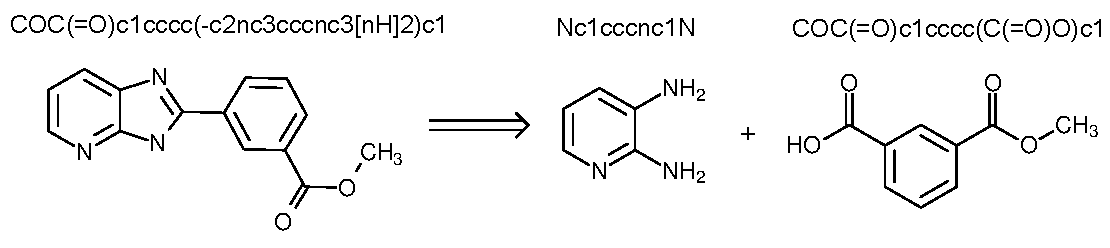
\includegraphics[scale=0.87]{images/example-reaction.pdf}
  \caption{An example of a retrosynthetic reaction: on the left side of the arrow the target molecule is depicted, and on the right side the one possible set of reactants that can lead to the target is shown in common chemistry-like scheme and using SMILES notation. Here two successive amidation reactions result in cyclisation and aromatization.}
  \label{fig:example-reaction}
\end{figure}

Neural sequence-to-sequence (seq2seq) approach has been recently applied for a direct reaction 
prediction task \cite{SchwallerTranslation,SchwallerTransformer} with outstanding statistical 
parameters of final models -- 90.4\% of accuracy on test set. Seq2seq modeling has been also tested on 
retrosynthesis task\cite{Pande}, but due to the complex nature of retrosynthesis itself 
and difficulty in estimating the correct predictions of reactants
\footnote{A target molecule usually can be synthesized with different reactions starting from different sets of reactants. 
The predictions of the model may be correct from organic chemist point of view but differ from 
the reactant set in ground truth. This may lead to underestimation of effectiveness of models.}, 
accuracy on the test set was moderate 37.4\% but still comparable to rule-based systems 35.4\%. 
We questioned about the possibility of improvement models for one-step retrosynthesis utilizing modern neural network architectures 
and training techniques. Applying the Transformer Model\cite{Transformer}, 
together with cyclical learning rate schedule\cite{TransformerTips}, 
and knowledge distillation\cite{Hinton} resulted in a single model with accuracy 44.2\%, 
that is more than 6\% higher compare to the baseline model\cite{Pande}.  

Our main contributions are:
\begin{itemize}
\item We show that for this particular task there is no need to use a vliadation dataset for early-stopping or other parameters optimization. We trained all the parameters directly from the training dataset.
\item Applying weights averaging, snapshot learning and knowledge distillation helped us to train the most precise model for one-step retrosynthesis prediction.
\item We show that different chemistry-relevant SMILES tokenization approaches cannot improve the accuracy of the models compared to the simplest letter based schema. 
\item Increasing the temperature while performing a beam-search procedure improves the accuracy up to 4\%. Almost the same effect as consensus does. 
\item Using both retrosynthetic model for reactant prediction and a direct model trained on the same data for reaction outcome prognosis allows improving precision of the retrosynthesis model.
\end{itemize}

\section{Approach}
\label{sec:approach}

\subsection{Dataset}

In this study we used the same dataset of reactions as in \cite{Pande}. 
This dataset was filtered from the USPTO database\cite{Lowe} originally derived from the USA patents and 
contains 50\,000 reactions classified into 10 reaction types\cite{Schneider}. The authors\cite{Pande} further preprocessed the database by 
splitting multiple products reactions into multiple single products reactions. The resulting dataset contains 40\,029, 5\,004, and 5\,004 reactions for training, validation, and testing respectively. Information about the reaction type 
was discarded as we aimed at building a general model using SMILES of products and reactants only.


\subsection{Model input}
The seq2seq models were developed to support machine translation where the input is a sentence in one language, and the output is a sentence with approximately the same meaning but in another language. String nature of data implies some tokenization procedures similar to word2vec to be used for preprocessing the input. Most of works in cheminformatics dealing with SMILES tokenize the input with a regexp equal or similar to \cite{SchwallerTranslation}. 

\begin{quote}
\texttt{token\_regex = "(\textbackslash[[\textasciicircum \textbackslash]]+]|Br?|Cl?|N|O|S|P|F|I|b|c|n|o|s|p|\textbackslash(|\textbackslash)| \textbackslash.|=|\#|-|\textbackslash+|\textbackslash\textbackslash\textbackslash\textbackslash|\textbackslash/|:|\textasciitilde|@|\textbackslash?|>|\textbackslash*|\textbackslash\$|\textbackslash\%[0-9]\{2\}|[0-9])"}.
\end{quote}

Though such tokenization is more similar to way chemists think, it also has some drawbacks that confuse network by putting forward low represented molecular parts. For example, after applying this regexp to the database one can see some not frequent moieties such as [C@@], [C@@H], [S@@],[C@],[C@H],[N@@+],[se],[C-],[Cl+3]. The thing in brackets according to SMILES specification can be quite a complex gathering not only the element's name itself, but also its isotopic value, stereochemistry configuration, the formal charge, and the number of hydrogens\footnote{We do not want to exclude stereochemistry information from our model as well as charges and explicit hydrogens that will lead to reducing of the dataset. Moreover, work in generative models showed excellent abilities of models to close cycles, for example, c\textbf{1}cc(COC)cccc\textbf{1}. If the model can capture such a long distance relation why should it be cracked on much simplier substrings enclosed by brackets?}. Strictly speaking, to do tokenization right one should also parse the content of brackets just increasing the number of possible words in the vocabulary what eventually leads to the simplest tokenization only with letters. We tried different schemes of tokenization in this work but did not see any improvements in using them over character-based method.

Our final vocabulary has length of 66 symbols\footnote{This vocabulary derived from the complete USPTO set and is a little bit wider than needed for this study. But for future extending of the models it is better to fix the input shape to the biggest possible value.}:

\begin{quote}
\texttt{chars = " \textasciicircum\#\%()+-.\/0123456789=@ABCDEFGHIKLMNOPRSTVXYZ[\textbackslash\textbackslash]abcdefgilmnoprstuy\$"}
\end{quote}

To convert a token to a dense vector we used a trainable embedding
\footnote{The encoder and the decoder share embeddings in this study.} of size 64. 
It is well known that training neural networks in batches is more stable, faster, and leads to more accurate models. 
To facilitate batch training we also used masks of input strings of shape (batch\_size, max\_length) 
with elements equal to 1 for those positions where are valid SMILES symbols and 0 everywhere else. 


\subsection{Transformer model}
We used a promising Transformer \cite{Transformer} model for this study which is a new generation of encoder-decoder neural networks family. The architecture is suited for exploration of the internal representation of data by deriving questions ($Q$) the data could be asked for, keys for its indexed knowledge ($K$), and answers written as values ($V$) corresponding to queries and keys. Technically these three entities are simply matrixes learned during the network training. Multiplying them with the input ($X$) gives keys ($k$), questions ($q$), and values ($v$) relevant to a current batch. Equipped with these calculated parameters of the input the self-attention layers transforms it pointing out to some encoding (decoding) parts based on the attention vector. 

The Transformer has wholly got rid of any recurrences or convolutional operations. To tackle distances between elements of a string a positional encoding matrix was proposed with elements equal to the values of trigonometric functions depending on the position in a string and also the position in the embedding direction. Summed with learned embeddings positional encodings do their job linking far located parts of the input together. The output of self-attention layers is then mixed with original data, layer-wise normalized, and passed position-wise through a couple of ordinary dense layers to go further either in next level of self-attention layers or to a decoder as an information-rich vector representing the input. The decoder part of Transformer resembles the encoder but has an additional self-attention layer which corresponds to encoder's output. 

Transformer model shows the state-of-the-art results in machine translation and reaction prediction outcomes \cite{SchwallerTransformer}. The latter work showed that training the Transformer on large and noisy datasets results in a model that can outperform not only other machine models but also well qualified and experienced organic chemists. 

\subsection{Model inference}

The model tries to estimate the probability of the next symbol over the model's vocabulary given all previous symbols in the string. Technically, the Transformer model first calculates logits, $z_i$, and then transforms them to probabilities. 
\begin{equation}
z_i = Transformer( \{x_1, x_2, x_3, ..., x_L\}, \{y_1, y_2, y_3, ..., y_{i-1} \})
\end{equation}
Here $x_i$ is the input of the models at $i$ position; $L$ -- the length of the input string; $y_i$ is the decoded output of the model up to position $(i-1)$; and $z_i$ -- logits that are to be converted to probabilities:
\begin{equation}
\label{eq:tempdep}
q_i = {{exp(z_i /T) }\over {\sum_{j=0}^{V} exp(z_j /T) }}
\end{equation}
where $V$ is the size of the vocabulary (66 in this work) and $T$ stands for the temperature\footnote{Similar to formula of Boltzmann (Gibbs) distribution used in statistical mechanics.} usually assigned to 1.0 in standard softmax layers. With higher $T$ the landscape of the probability distribution becomes more smooth. During the training the model adapts its weights to better predict $q_i$, so $y_i = q_i$. 

During the inference however we have several possibilities how to convert $q_i$ into $y_i$, namely greedy and beam search. The first one picks up a symbol with maximum probability whereas the second one at each step holds $top-K$ ($K$ = beam's size) suggestions of the model and summarises the overall likelihood for each of $K$ final decodings. The beam search allows better inference and the probability landscape exploration compared to the greedy search because at a particular step of decoding it may choose a symbol with less than maximum probability, but the total likelihood of the result can be higher due to more significant probabilities on the next steps.

\subsection{Training heuristics}
Training a Transformer model is a challenge, and several heuristics have been proposed\cite{TransformerTips}, some of them were used in this study:

\paragraph{Using as bigger batch size as possible.} However, due to our hardware limitations we could not set the batch size more then 64\footnote{Our first implementation of the model required a lot of memory to deal with masks of reactants and products. Though later we improved the code we still remained this size for consistency of the results.};
\paragraph{Iincreasing the learning rate at the beginning} of training up to warmup steps\footnote{In our implementation 1 step is equivalent to 1 batch. The number of reactions for training is 40\,029 + 5\,004, so one epoch is equal to 704 batches.}. The authors of the original Transformer paper \cite{Transformer}  used 4\,000 steps for warming. The Transformer model for reaction prediction task from \cite{SchwallerTransformer} used 8\,000 steps. We have also tried different values for warmup and eventually found that 16\,000 works well with our model.
\paragraph{Applying cyclic learning rate} schedules. This tips can generally improve any model\cite{Izmailov} through better loss landscape exploration with bigger learning rates after the optimiser felt down to some local minima. For this study we used the following scheme for learning rate calculation depending on the step:
\[
    u(step)= 
\begin{cases}
    warmup + (step \bmod cycle), & \text{if } step \ge cycle\\
    step,              & \text{otherwise}
\end{cases}
\]
where $cycle$ stands for the number of steps while the learning rate is decreasing before raising to the maximum again.
\begin{equation}
\label{eq:rate}
\lambda(step) = factor * { {min (1.0, u(step) / warmup ) } \over { max (u(step), warmup) } }
\end{equation}	
where $factor$ is just a constant. Big values of $factor$ introduce numerical instability during training, so after several trials we set $factor = 20.0$. The curve for learning rate in this study is shown in fig. \ref{fig:example}, plot (4, f).
\paragraph{Averaging weights} during last steps (usually 10- 20) of training or at minima of learning rates in case of snapshop learning \cite{Snapshot}.

\subsection{Knowledge distillation}
After training a (teacher) model it is possible to get predictions for the training set and then train another (student) model on these predictions. This second model usually outperforms the first one. This approach was further developed in\cite{Hinton} where the algorithm for knowledge distillation was proposed. The key idea is to calculate probabilities for training dataset at higher temperature $T$, eq. \ref{eq:tempdep}, and then use this values as targets along with the correct labels. The final loss function:
\begin{equation}
\label{eq:hard}
Loss = -\sum y log(q) - T^2 * \sum q_{teacher} log(q)  
\end{equation}
contains terms for hard and soft labels and, thus, the model will learn to distinguish subtle differences in final probability distribution. We applied this technique for further training our models and found that this simple approach can improve the accuracy up to 2\%.

\section{Results}
\label{sec:results}

\begin{wrapfigure}{r}{7cm}  
  \vspace{-0.5cm}
  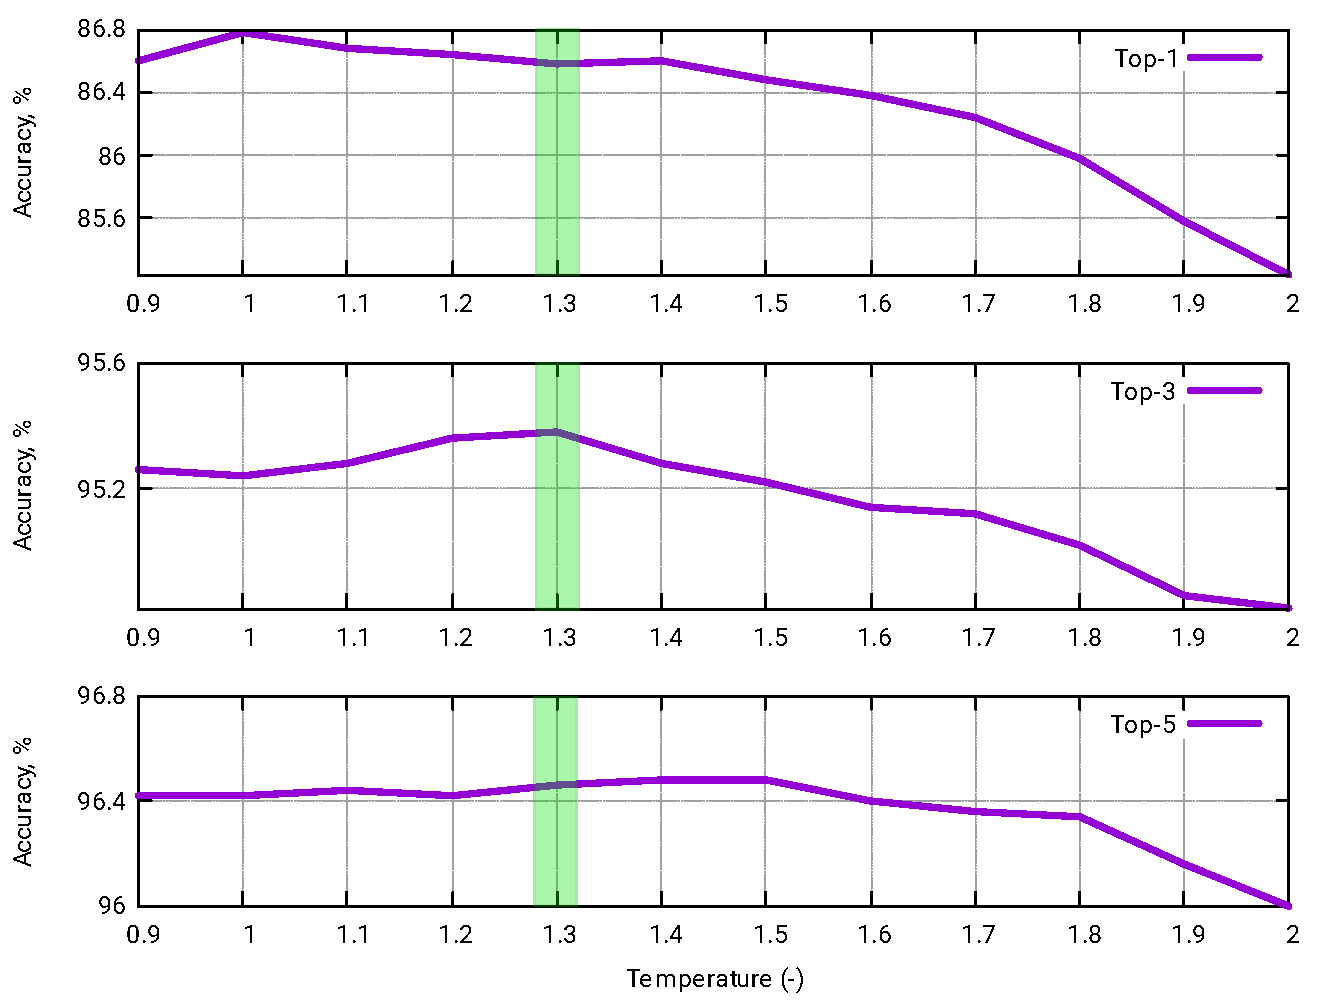
\includegraphics[width = 7cm]{images/tempdep.pdf}
  \caption{Dependence of the beam search on temperature. For better exploration, higher temperatures are more useful. In this study we explored T=1.3. Bigger values significantly worse for Top-3, and approximately the same for Top-1 and Top-5. This curve was derived from the training dataset.}
  \label{fig:tempdep}
  \vspace{-0.2cm}
\end{wrapfigure}
For this study, we implemented The Transformer model in Tensorflow library to support its integration in our in-house programs set (\url{https://github.com/bigchem/retrosynthesis}).  All values reported are averages for three repetitive runs. Preliminary modeling showed that the architecture with 3 layers and 8 attention heads works well for the datasets, though we tried combinations of 2, 3, 4, 5 layers with 6, 8, 10, 12 heads. So all calculations were performed with these values fixed.  The number of learnable parameters of the model is 1\,882\,176, embedding layer common for product and reactants has size 64.
\begin{table}[b!]
  \caption{Accuracy (\%) of the models on test set when all reactants were correctly predicted.}
  \centering
  \begin{tabular}{p{2cm}p{1cm}p{1cm}p{1cm}p{1cm}p{8cm}}
    \toprule
    Model & Greedy & Top-1 & Top-3 & Top-5 & Description\\
    \midrule
    Seq2Seq &  & 37.4  & 52.4 & 57.0 & Literature result from \cite{Pande} based on Seq2Seq architecture. \\ \midrule
    T1         & 34.4 & 37.9 & 57.3 & 62.7 & Transformer Model trained with validation control set (early stopping, \textasciitilde 200 epochs). \\
    T$1_1$ & 37.3 & 39.8 & 59.1 & 63.9 & The same as T1, but without early stopping (1000 epochs). \\ 
    T2         & 39.3 & 41.8 & 61.3 & 67.2 & Transformer Model trained on both training and validation sets for 1000 epochs.\\
    T3         & 40.6 & 42.7 & 63.9 & 69.8 & Transformer Model trained with cyclic learning rate schedule for 1000 epochs. Averaging cycles 6,7,8,10.\\
    T4         & &  &  &  & Transformer Model trained with distillation approach \cite{Hinton} for 1000 epochs.\\ 
    \bottomrule
  \end{tabular}
  \label{tbl:results}
\end{table}

Following the standard machine learning protocol, we trained our first models (T1) using three datasets for training, validation, and external testing (8:1:1) as was done in \cite{Pande}. Learning curves for T1 are depicted in fig. \ref{fig:example}, (d) and (e) for training and validation loss, respectively, (g) shows the original learning rate schedule developed by the authors of the Transformer but with 16\,000 warmup steps. On reaching cross-entropy loss about 0.1 on the validation dataset, it stagnates without noticeable fluctuations as training loss steadily decreases. After warming up phase the learning rate begins fading and eventually after 1\,000 epochs its value reaches $2.8*10^{-5}$ inevitable causing to stop training because of too small updates. 

During the decoding procedure, we explored the influence of the temperature parameter on the final quality of prediction and surprisingly found that inferring at higher temperatures gives better result then at T=1. This observation similarly repeated for all our models. Fig. \ref{fig:tempdep} shows the influence of this parameter on the reactants prediction of the part of the training set. Clearly, at T=1.3 the model reaches the maximum of chemically-based accuracy. This fact one can explain that at higher temperatures the landscape of output probabilities of the model is softer letting the beam-search procedure to find more suitable ways during decoding. Of course, the temperature influences only relative distances between peaks, so it does not affect the greedy search method. 

If we apply the early stopping technique, we should select the model around 200 epoch. Effectiveness of such a model marked $T1_1$ in table \ref{tbl:results} resulted in TOP-1 40.16\% on the test set. If we choose the last one model obtained at 1\,000 epoch, then the model $T1_2$ gives us slightly better values. In this case, we did not see any need of the validation dataset and keeping in mind that our model has almost 2 millions of parameters we decided to combine training and validation sets and train our next models on both data, e.g., without validation. The model $T2$ was trained on all data and with the same learning rate schedule as $T1$. The results obtained when applying T2 to the test set are better than for T1 set.

Then we trained our model with cyclic learning rate schedule, eq. \ref{eq:rate}, fig. \ref{fig:example} (f) for better exploration of loss landscape. During training, we also saved the character-based accuracy of the model, fig. (b). This snapshot training regime \cite{Snapshot} produces a set of different weights at each minimum of learning rate. Averaging them is to some extent equivalent to a consensus of models but within one model \cite{Izmailov}. We tried different averaging regimes $T3_{2-3}$ but did not see any remarkable improvements. 
\begin{figure}[t!]
  \centering
  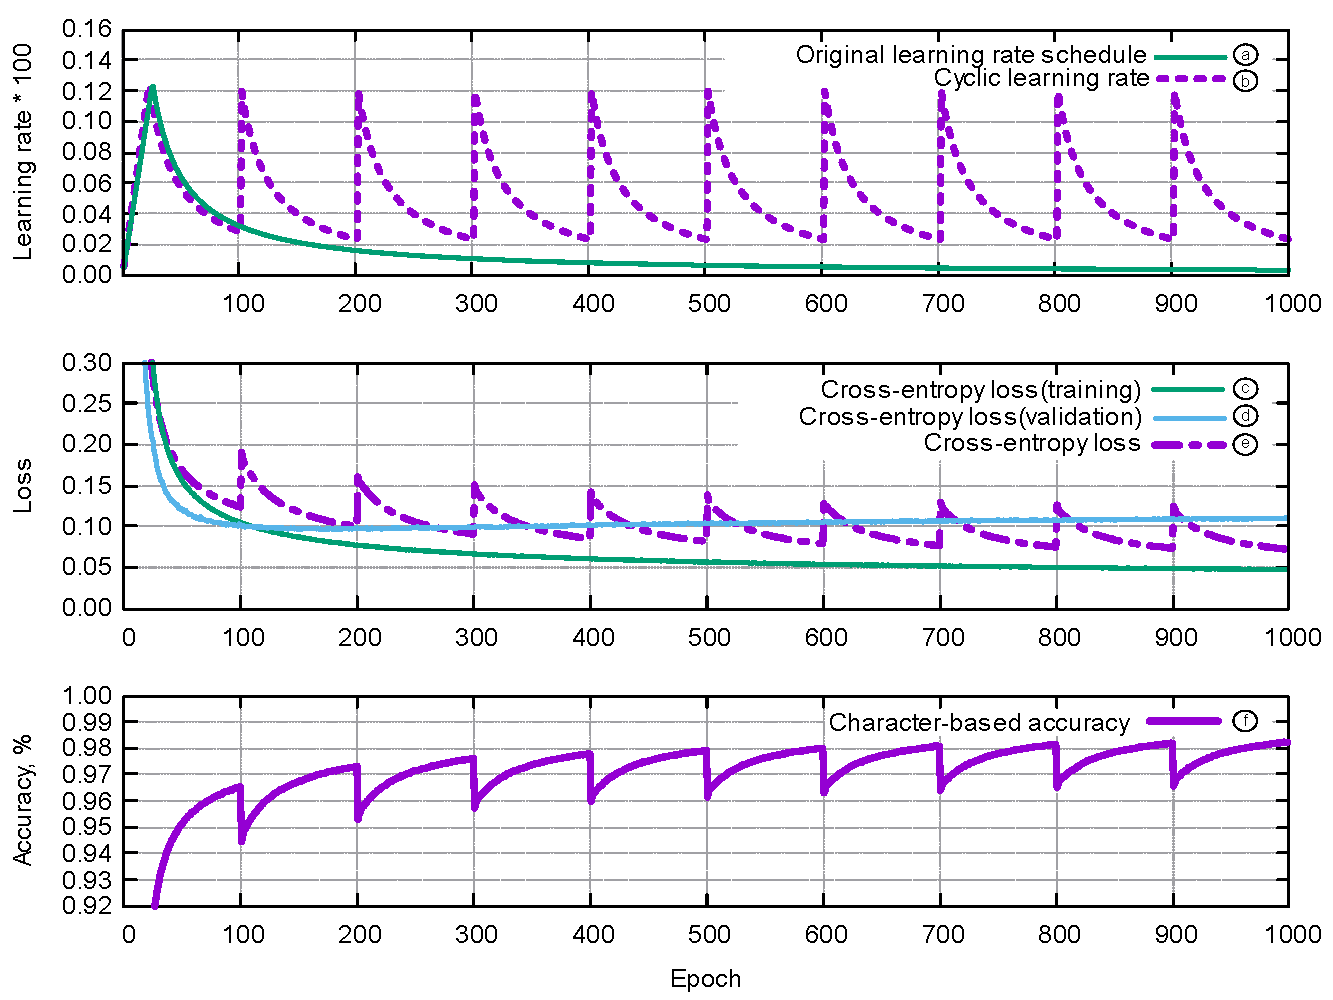
\includegraphics[width = 17cm]{images/learning.pdf}
  \caption{Summary of learning curves for the Transformer model: 1) Accuracy of correctly predicted reactants in test set (a); 2) character based accuracy (b); 3) cross-entropy loss with cycling learning rate (f) for the entire dataset (c) and losses for training (d) and validation (e) sets with monotonically decreasing learning rate (g); 4) learning rate schedules as a function of epoch.}
  \label{fig:example}
\end{figure}

Our T3 model outperforms \cite{Pande} by 3.8\% with beam search and more critical by 3.0\% with the greedy search. The latter one is much faster and consequently more suitable for virtual screening campaigns. To improve the quality of this model, we applied the knowledge distillation approach. First, the soft labels were calculated using T3 model, and, second, we traing T4 model from scratch but with two terms in the objective function: one for hard and one for soft labels, eq. \ref{eq:hard}. 


\section{Discussion}

Some discussion...

\begin{figure}
  \centering
  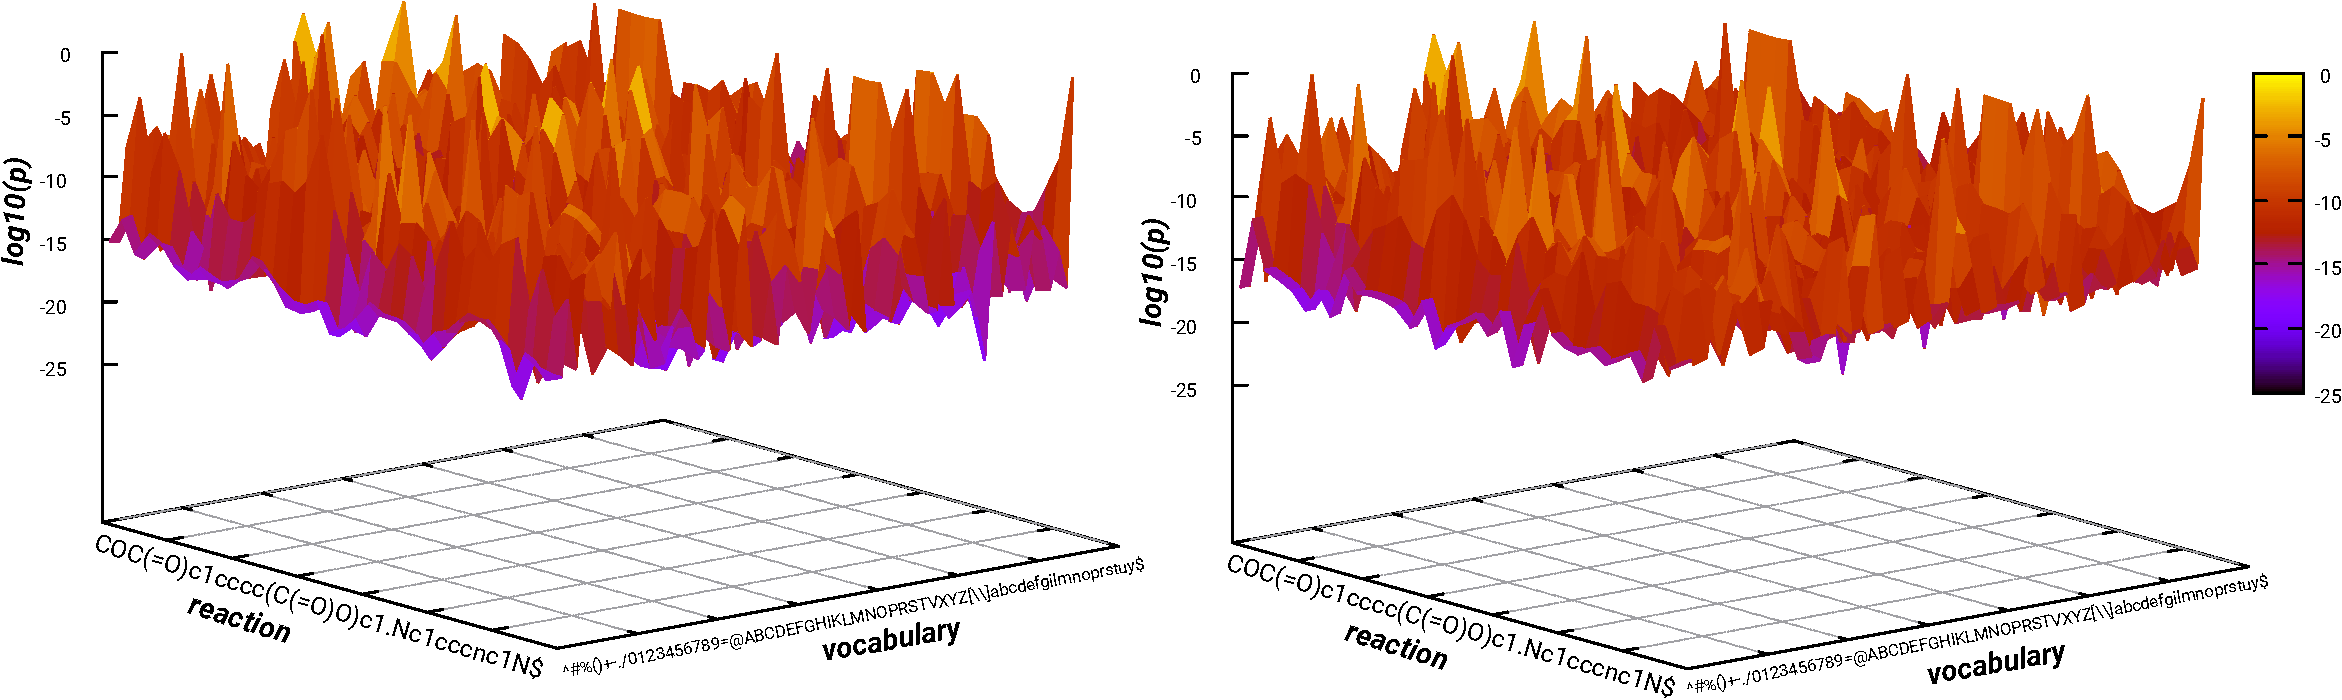
\includegraphics[width = 16.5cm]{images/probland.pdf}
  \caption{Landscapes of probabilities for predicting example reaction, fig. \ref{fig:example}, with  T3 model(left) and T4 (distilled) model (right). }
  \label{fig:landscape}
\end{figure}

All source code and also models built are available online via github
\begin{center}
  \url{https://github.com/bigchem/retrosynthesis}
\end{center}

\section*{Acknowledgments}
This study has been partially supported by ERA-CVD (\url{httpd://era-cvd.eu}) "Cardio-Oncology" project, BMBF 01KL1710.
The authors thank NVIDIA Corporation for donating Quadro P6000 and Titan Xp graphics cards for this research.

\bibliographystyle{naturemag}  
\bibliography{references}
 
 \newpage
 
\section{Appendix}

In this section we report all characteristics of repetitive runs of all models built in this study. Average values based on this data are summed in table \ref{tbl:results}. For every run we report learning curves with loss functions and learning rate, then model relevant information are collected in a table including greedy search decoding accuracies, beam search accuracies for Top-1, Top-3, and Top-5.

\subsection{Model 1} 
\subsubsection{Model 1 (run-1)}
  
\begin{figure}[h!]
  \centering
  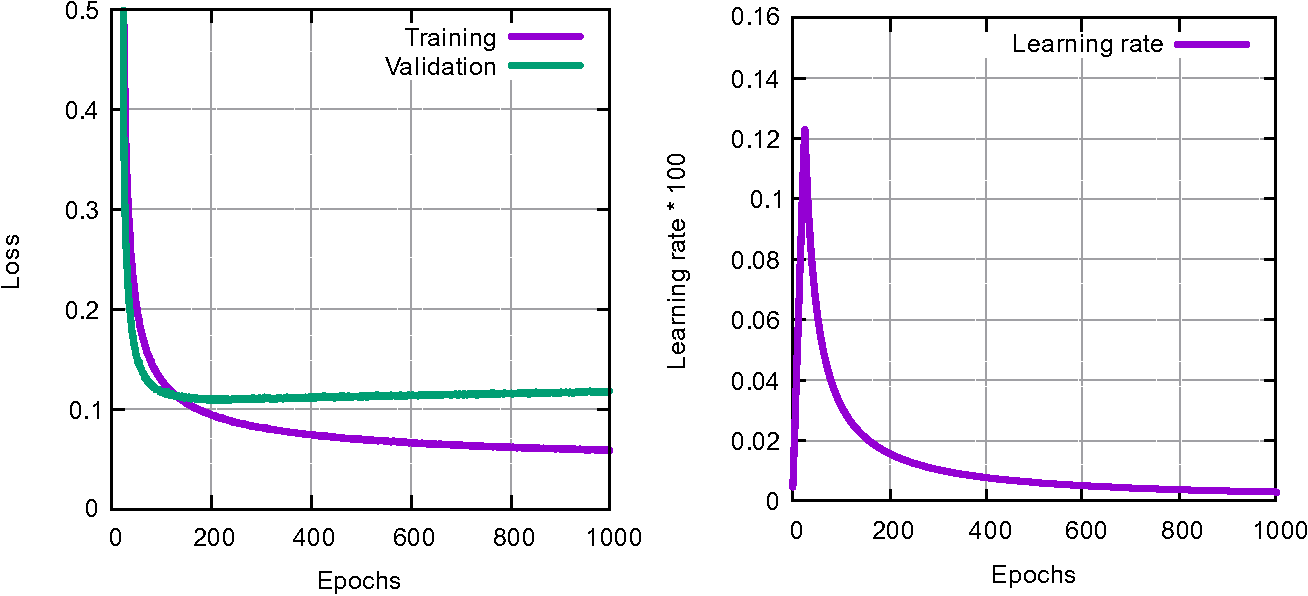
\includegraphics[width = 16.5cm]{images/t1-1.pdf}
  \caption{Learning curves and rate schedule for T1 model. Losses for training and validation datasets on the left, usual learning rate schedule on the right.}
  \label{fig:t11}
\end{figure}

\begin{table}[h!]
\caption{Parameters of T11 run.}
  \centering
  \begin{tabular}{p{6.2cm}p{3.5cm}p{1.5cm}p{1.5cm}p{1.5cm}}
    \toprule
    Parameter & Value & Top-1 & Top-3 & Top-5 \\
    \midrule
    Early stopping loss (training / validation) &  0.09345 / 0.10864 & & & \\
    Last training loss (training / validation) &  0.05867 / 0.11819& & & \\
    Epoch (early stopping) & 208 & & & \\
    \midrule
    Greedy search (early stopping, epoch 208) & & 32.83 & &\\
    Greedy search (last, epoch 999) & & 34.75 & & \\
    Greedy (last 10 average, epoch, 990 - 999) & & 35.57 & & \\
    \midrule
    Beam, T = 1.0 (early) & & 35.57 & 54.14 & 59.13 \\
    Beam, T = 1.3 (early) & & 35.93 & 54.59 & 59.51 \\ 
    \midrule
    Beam, T = 1.0 (last) & & 37.15 & 55.22 &  60.49 \\
    Beam, T = 1.3 (last) & & 37.67 & 55.97 & 61.01 \\ 
    \midrule
    Beam, T = 1.0 (last 10 average) & & 37.83 & 56.08 &  60.63 \\
    \textbf{Beam, T = 1.3 (last 10 average)}  & & \textbf{38.15} & \textbf{56.71} & \textbf{61.31} \\ 
    \bottomrule
  \end{tabular}
  \label{tbl:t11}

\end{table} 


\url{https://github.com/bigchem/retrosynthesis/papers/retrosynthesis/models/t1-1-early.h5}

\url{https://github.com/bigchem/retrosynthesis/papers/retrosynthesis/models/t1-1-last.h5}

\url{https://github.com/bigchem/retrosynthesis/papers/retrosynthesis/models/t1-1-avg.h5}


\newpage

\subsubsection{Model 1 (run-2)}
  
\begin{figure}[h!]
  \centering
  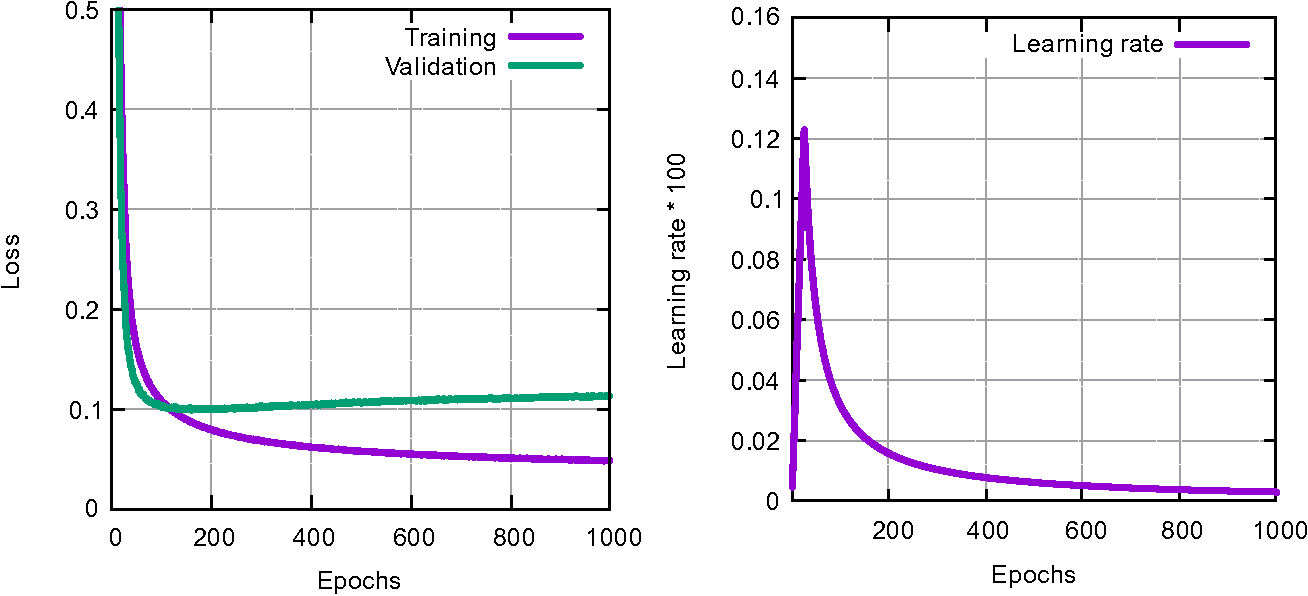
\includegraphics[width = 16.5cm]{images/t12.pdf}
  \caption{Learning curves and rate schedule for T1 model. Losses for training and validation datasets on the left, usual learning rate schedule on the right.}
  \label{fig:t11}
\end{figure}

\begin{table}[h!]
\caption{Parameters of T12 run.}
  \centering
  \begin{tabular}{p{6.2cm}p{3.5cm}p{1.5cm}p{1.5cm}p{1.5cm}}
    \toprule
    Parameter & Value & Top-1 & Top-3 & Top-5 \\
    \midrule
    Early stopping loss (training / validation) &  0.08681 / 0.09926 & & & \\
    Last training loss (training / validation) &  0.04863 / 0.11316  & & & \\
    Epoch (early stopping) & 162 & & & \\
    \midrule
    Greedy search (early stopping, epoch 162) &  & 34.63 & &\\
    Greedy search (last, epoch 990) &  & 38.07  & & \\
    Greedy (last 10 average, epoch, 990 - 999) & & 38.19 & & \\
    \midrule
    Beam, T = 1.0 (early) & & 37.45 & 56.71 & 62.43 \\
    Beam, T = 1.3 (early) & & 38.31 & 57.93 & 63.35 \\ 
    \midrule
    Beam, T = 1.0 (last) & & 39.83 & 58.63 &  64.45 \\
    Beam, T = 1.3 (last) & & 40.67 &  59.53 & 64.97 \\ 
    \midrule
    Beam, T = 1.0 (last 10 average) & & 40.22 & 59.05 &  64.91 \\
    \textbf{Beam, T = 1.3 (last 10 average)} & & \textbf{40.85} &  \textbf{59.85} & \textbf{65.45} \\ 
    \bottomrule
  \end{tabular}
  \label{tbl:t12}

\end{table} 

\url{https://github.com/bigchem/retrosynthesis/papers/retrosynthesis/models/t1-2-early.h5}

\url{https://github.com/bigchem/retrosynthesis/papers/retrosynthesis/models/t1-2-last.h5}

\url{https://github.com/bigchem/retrosynthesis/papers/retrosynthesis/models/t1-2-avg.h5}

\newpage

\subsubsection{Model 1 (run-3)}
  
\begin{figure}[h!]
  \centering
  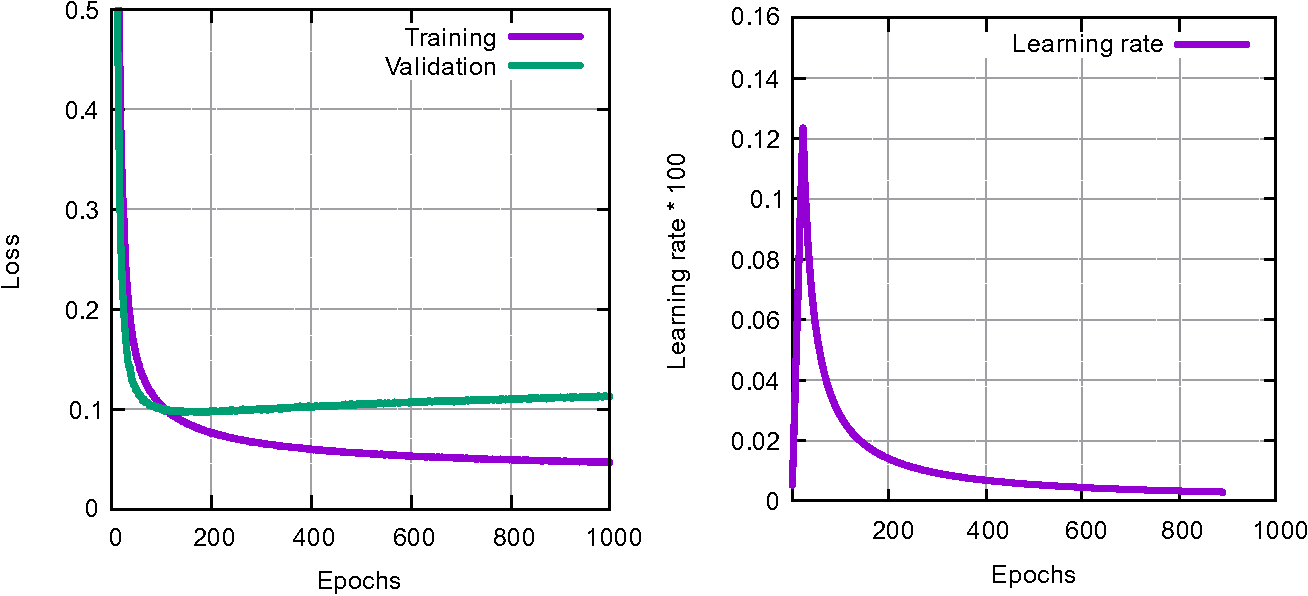
\includegraphics[width = 16.5cm]{images/t1-3.pdf}
  \caption{Learning curves and rate schedule for T1 model. Losses for training and validation datasets on the left, usual learning rate schedule on the right.}
  \label{fig:t11}
\end{figure}

\begin{table}[h!]
\caption{Parameters of T13 run.}
  \centering
  \begin{tabular}{p{6.2cm}p{3.5cm}p{1.5cm}p{1.5cm}p{1.5cm}}
    \toprule
    Parameter & Value & Top-1 & Top-3 & Top-5 \\
    \midrule
    Early stopping loss (training / validation) &  0.07795 / 0.09662 & & & \\
    Last training loss (training / validation) &  0.04654 / 0.11285  & & & \\
    Epoch (early stopping) & 193 & & & \\
    \midrule
    Greedy search (early stopping, epoch 193) &  & 35.63 & &\\
    Greedy search (last, epoch 998) &  & 38.13 & & \\
    Greedy (last 10 average, epoch, 990 - 999) & & 38.03 & & \\
    \midrule
    Beam, T = 1.0 (early) & & 38.75 & 58.55 &  64.47 \\
    Beam, T = 1.3 (early) & & 39.53 & 59.25 & 65.23 \\ 
    \midrule
    Beam, T = 1.0 (last) & & 40.05 & 59.35 &  64.27 \\
    Beam, T = 1.3 (last) & & 40.41 & 60.49 &  64.85 \\ 
    \midrule
    Beam, T = 1.0 (last 10 average) & & 39.96 & 59.83 & 64.46  \\
    \textbf{Beam, T = 1.3 (last 10 average)} & & \textbf{40.41}  & \textbf{60.81} & \textbf{65.18}  \\ 
    \bottomrule
  \end{tabular}
  \label{tbl:t13}

\end{table} 

\url{https://github.com/bigchem/retrosynthesis/papers/retrosynthesis/models/t1-3-early.h5}

\url{https://github.com/bigchem/retrosynthesis/papers/retrosynthesis/models/t1-3-last.h5}

\url{https://github.com/bigchem/retrosynthesis/papers/retrosynthesis/models/t1-3-avg.h5}

\newpage
\subsection{Model 2}
\subsubsection{Model 2 (run-1)}
 
\begin{figure}[h!]
  \centering
  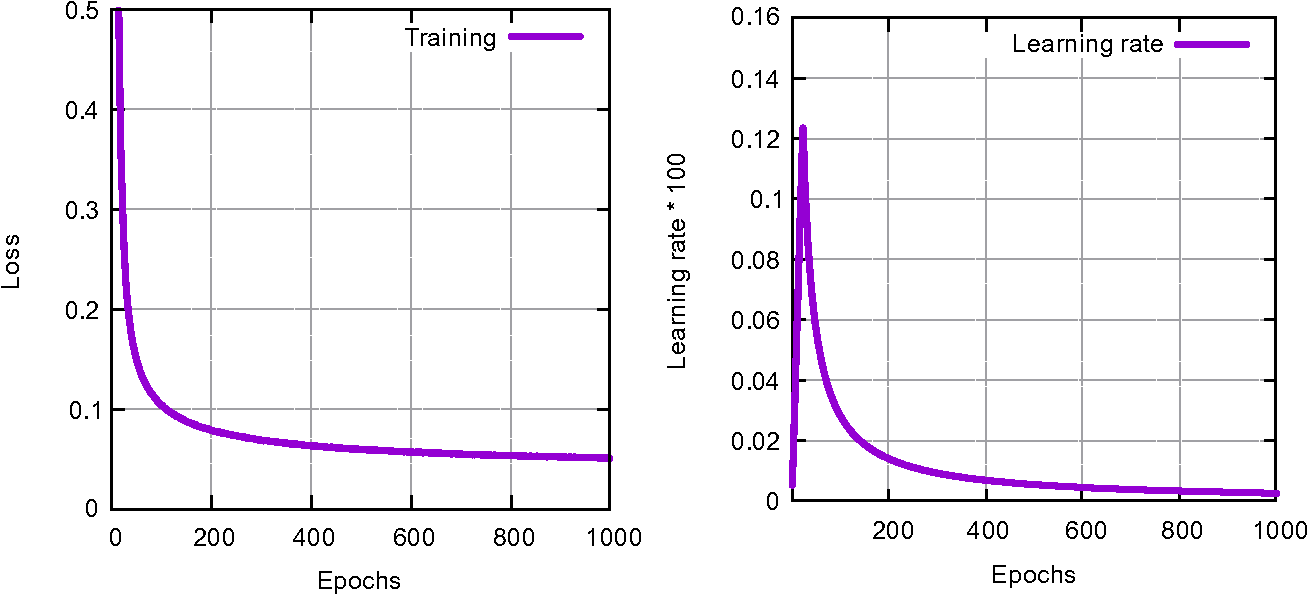
\includegraphics[width = 16.5cm]{images/t2-1.pdf}
  \caption{Learning curves and rate schedule for T2 model. Loss for training on the left, usual learning rate schedule on the right.}
  \label{fig:t21}
\end{figure}

\begin{table}[h!]
\caption{Parameters of T21 run.}
  \centering
  \begin{tabular}{p{8.2cm}p{1.5cm}p{1.5cm}p{1.5cm}p{1.5cm}}
    \toprule
    Parameter & Value & Top-1 & Top-3 & Top-5 \\
    \midrule
    Last training loss & 0.05108 & & & \\
    \midrule
    Greedy search (last, epoch 981) & & 38.85 & & \\
    Greedy (last 10 average, epoch, 990 - 999) & & 39.25 & & \\
    \midrule
    Beam, T = 1.0 (last) & & 40.57 &60.19  & 66.77 \\
    Beam, T = 1.3 (last) & & 41.17 & 60.65 &  67.28 \\ 
    \midrule
    Beam, T = 1.0 (last 10 average) & & 40.98 & 60.29 & 67.00 \\
    \textbf{Beam, T = 1.3 (last 10 average)} & &  \textbf{41.61} & \textbf{60.85} & \textbf{67.37} \\ 
    \bottomrule
  \end{tabular}
  \label{tbl:t21}

\end{table} 

\url{https://github.com/bigchem/retrosynthesis/papers/retrosynthesis/models/t2-1-last.h5}

\url{https://github.com/bigchem/retrosynthesis/papers/retrosynthesis/models/t2-1-avg.h5}

\newpage
 \subsubsection{Model 2 (run-2)}
 
\begin{figure}[h!]
  \centering
  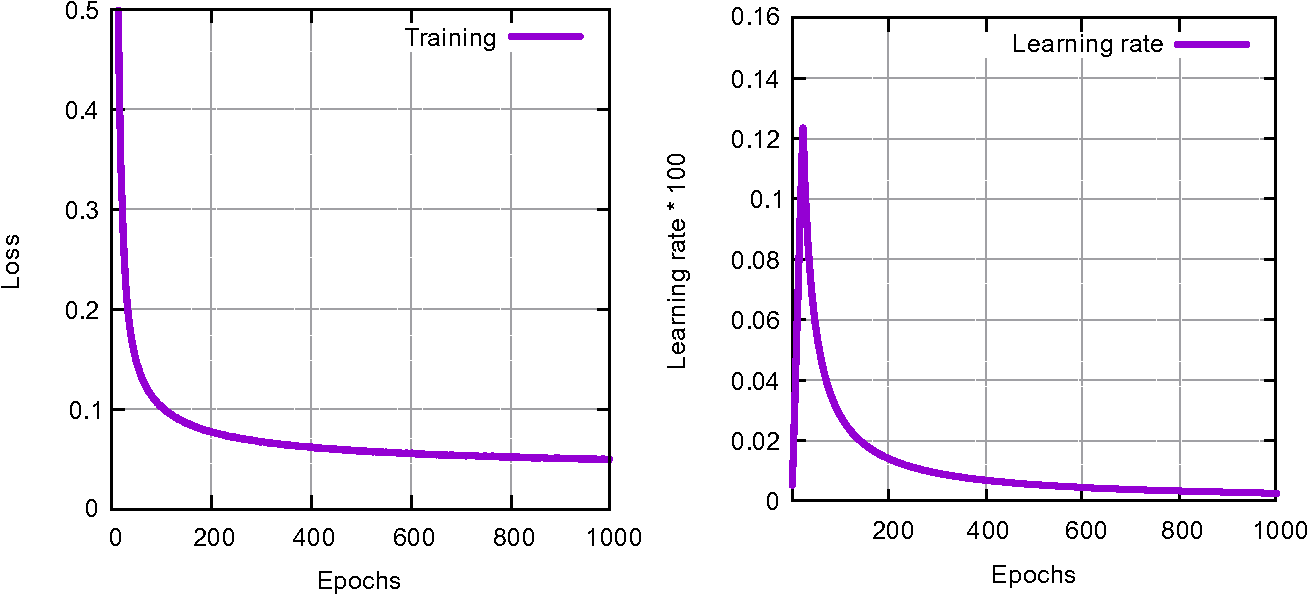
\includegraphics[width = 16.5cm]{images/t2-2.pdf}
  \caption{Learning curves and rate schedule for T2 model. Loss for training on the left, usual learning rate schedule on the right.}
  \label{fig:t21}
\end{figure}

\begin{table}[h!]
\caption{Parameters of T22 run.}
  \centering
  \begin{tabular}{p{8.2cm}p{1.5cm}p{1.5cm}p{1.5cm}p{1.5cm}}
    \toprule
    Parameter & Value & Top-1 & Top-3 & Top-5 \\
    \midrule
    Last training loss & 0.04943 & & & \\
    \midrule
    Greedy search (last, epoch 996) & & 38.79 & & \\
    Greedy (last 10 average, epoch, 990 - 999) & & 39.11 & & \\
    \midrule
    Beam, T = 1.0 (last) & & 40.98 & 60.39 & 66.38  \\
    Beam, T = 1.3 (last) & & 41.58 &  61.21 & 66.94 \\ 
    \midrule
    Beam, T = 1.0 (last 10 average) & & 41.14  & 60.59 &  66.41\\
    \textbf{Beam, T = 1.3 (last 10 average)} & &  \textbf{41.87} &  \textbf{61.35} &  \textbf{67.08}\\ 
    \bottomrule
  \end{tabular}
  \label{tbl:t22}

\end{table} 

\url{https://github.com/bigchem/retrosynthesis/papers/retrosynthesis/models/t2-2-last.h5}

\url{https://github.com/bigchem/retrosynthesis/papers/retrosynthesis/models/t2-2-avg.h5}

\newpage
 \subsubsection{Model 2 (run-3)}
 
\begin{figure}[h!]
  \centering
  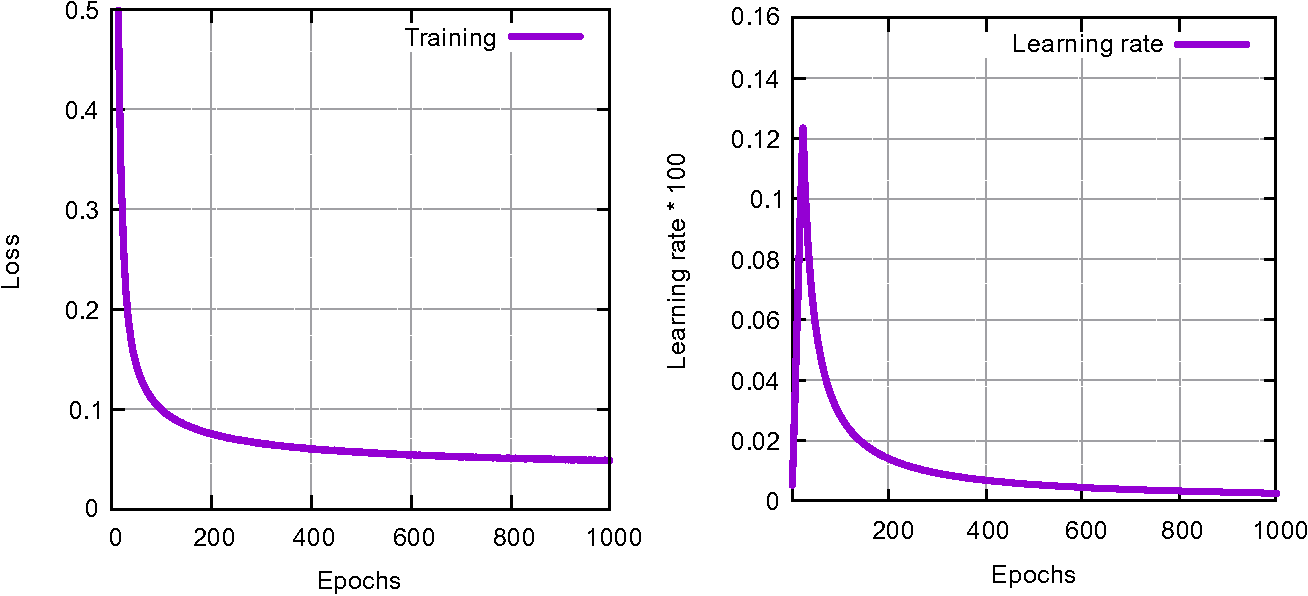
\includegraphics[width = 16.5cm]{images/t2-3.pdf}
  \caption{Learning curves and rate schedule for T2 model. Loss for training on the left, usual learning rate schedule on the right.}
  \label{fig:t21}
\end{figure}

\begin{table}[h!]
\caption{Parameters of T23 run.}
  \centering
  \begin{tabular}{p{8.2cm}p{1.5cm}p{1.5cm}p{1.5cm}p{1.5cm}}
    \toprule
    Parameter & Value & Top-1 & Top-3 & Top-5 \\
    \midrule
    Last training loss & 0.04826 & & & \\
    \midrule
    Greedy search (last, epoch 984) & & 39.79 & & \\
    Greedy (last 10 average, epoch, 990 -  999) & & 39.69 & & \\
    \midrule
    Beam, T = 1.0 (last) & & 41.55 & 60.79 & 66.57  \\
    Beam, T = 1.3 (last) & & 41.85 & 61.63  & 67.32 \\ 
    \midrule
    Beam, T = 1.0 (last 10 average) & & 41.45  & 60.75 &  66.55\\
    \textbf{Beam, T = 1.3 (last 10 average)} & & \textbf{42.02}  & \textbf{61.73}  & \textbf{67.19} \\ 
    \bottomrule
  \end{tabular}
  \label{tbl:t23}

\end{table} 

\url{https://github.com/bigchem/retrosynthesis/papers/retrosynthesis/models/t2-3-last.h5}

\url{https://github.com/bigchem/retrosynthesis/papers/retrosynthesis/models/t2-3-avg.h5}
 
 \newpage

 \subsection{Model 3}
 
 \subsubsection{Model 3 (run-1)}
 
\begin{figure}[h!]
  \centering
  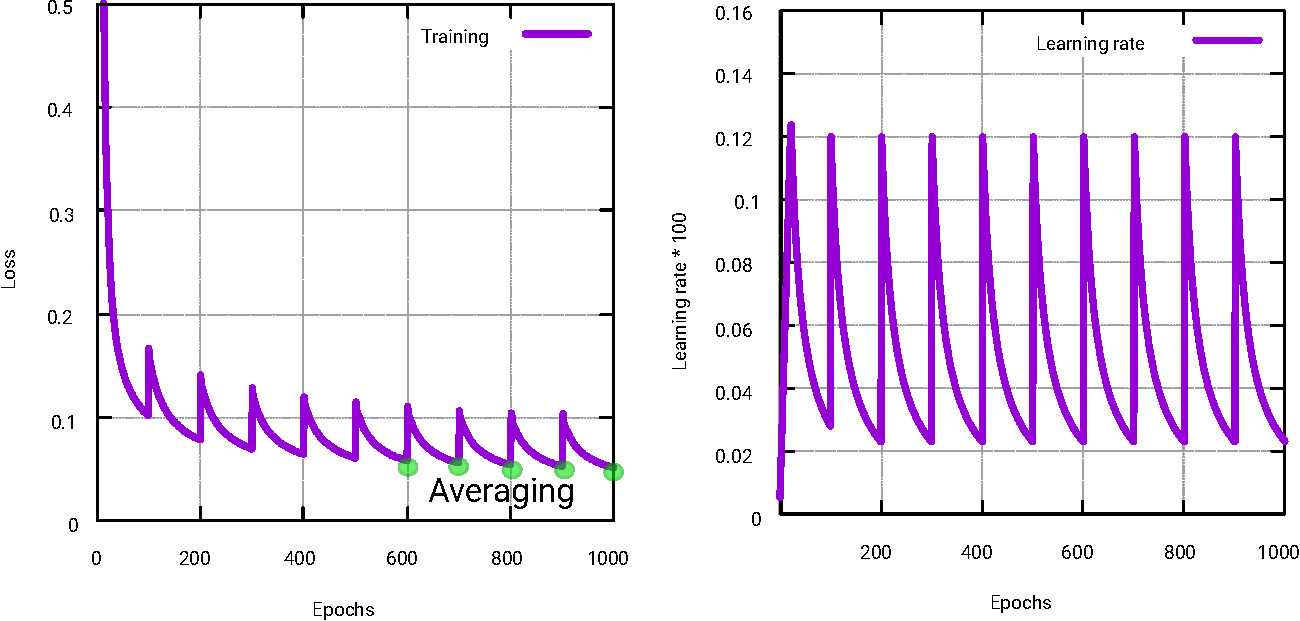
\includegraphics[width = 16.5cm]{images/t3-1.pdf}
  \caption{Learning curves and rate schedule for T3 model. Loss for training on the left, usual learning rate schedule on the right.}
  \label{fig:t11}
\end{figure}

\begin{table}[h!]
\caption{Parameters of T31 run.}
  \centering
  \begin{tabular}{p{8.2cm}p{1.5cm}p{1.5cm}p{1.5cm}p{1.5cm}}
    \toprule
    Parameter & Value & Top-1 & Top-3 & Top-5 \\
    \midrule
    Last training loss & 0.05173 & & & \\
    \midrule
    \multicolumn{5}{l}{\textbf{Averaging 6-7-8-9-10}} \\ \midrule
    Greedy search  & & 40.92 & & \\
    Beam, T = 1.0  & & 42.38 & 62.77 & 69.58  \\
    Beam, T = 1.3 & & 42.80 & \textbf{63.82} & 70.28 \\ 
    \midrule
    \multicolumn{5}{l}{Averaging 7-8-9-10} \\ \midrule
    Greedy search  & & 40.50 & & \\
    Beam, T = 1.0  & & 42.38 & 62.91 & 69.76  \\
    Beam, T = 1.3 & & 42.84 & 63.62 & 70.06 \\ \midrule
    \multicolumn{5}{l}{Averaging 8-9-10} \\ \midrule
    Greedy search  & & 41.04 & & \\
    Beam, T = 1.0  & &  &  &   \\
    Beam, T = 1.3 & &  &  &  \\ \midrule
    \multicolumn{5}{l}{Averaging 9-10} \\ \midrule
    Greedy search  & &  & & \\
    Beam, T = 1.0  & &  &  &   \\
    Beam, T = 1.3 & &  &  &  \\ 
    \bottomrule
  \end{tabular}
  \label{tbl:t31}
\end{table} 

Model with weights averaging 6-7-8-9-10:

\url{https://github.com/bigchem/retrosynthesis/papers/retrosynthesis/models/t3-1.h5}

\newpage
 
\subsubsection{Model 3 (run-2)}
 
\begin{figure}[h!]
  \centering
  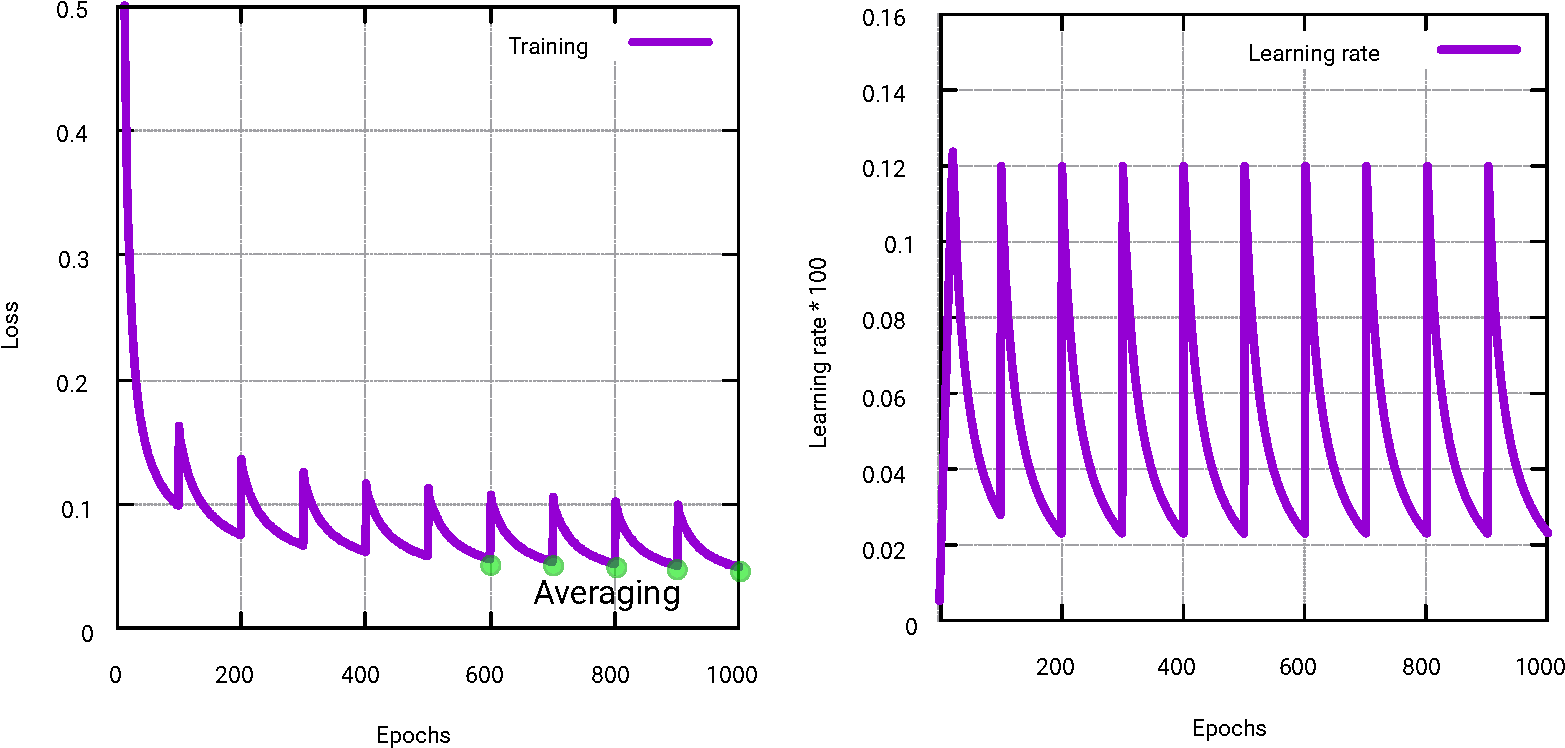
\includegraphics[width = 16.5cm]{images/t3-2.pdf}
  \caption{Learning curves and rate schedule for T3 model. Loss for training on the left, usual learning rate schedule on the right.}
  \label{fig:t11}
\end{figure}

\begin{table}[h!]
\caption{Parameters of T32 run.}
  \centering
  \begin{tabular}{p{8.2cm}p{1.5cm}p{1.5cm}p{1.5cm}p{1.5cm}}
    \toprule
    Parameter & Value & Top-1 & Top-3 & Top-5 \\
    \midrule
    Last training loss & 0.04958 & & & \\
    \midrule
    \multicolumn{5}{l}{\textbf{Averaging 6-7-8-9-10}} \\ \midrule
    Greedy search  & & 40.32 & & \\
    Beam, T = 1.0  & & 41.90 & 62.70 & 68.80  \\
    Beam, T = 1.3 & & 42.42 & \textbf{63.61} & 69.66 \\ 
    \midrule
    \multicolumn{5}{l}{Averaging 7-8-9-10} \\ \midrule
    Greedy search  & & 40.22 & & \\
    Beam, T = 1.0  & & 41.90 & 62.72 & 69.18  \\
    Beam, T = 1.3 & & 42.42 & 63.59 & 69.92 \\ \midrule
    \multicolumn{5}{l}{Averaging 8-9-10} \\ \midrule
    Greedy search  & & 40.56 & & \\
    Beam, T = 1.0  & & 41.96 & 62.53 & 69.18  \\
    Beam, T = 1.3 & & 42.62 & 63.14 & 69.86 \\ \midrule
    \multicolumn{5}{l}{Averaging 9-10} \\ \midrule
    Greedy search  & & 40.34 & & \\
    Beam, T = 1.0  & & 41.98 & 62.43 & 69.14  \\
    Beam, T = 1.3 & & 42.34 & 63.03 & 69.70 \\ 
    \bottomrule
  \end{tabular}
  \label{tbl:t32}
\end{table} 

Model with weights averaging 6-7-8-9-10:

\url{https://github.com/bigchem/retrosynthesis/papers/retrosynthesis/models/t3-2.h5}
\newpage


\subsubsection{Model 3 (run-3)}
 
\begin{figure}[h!]
  \centering
  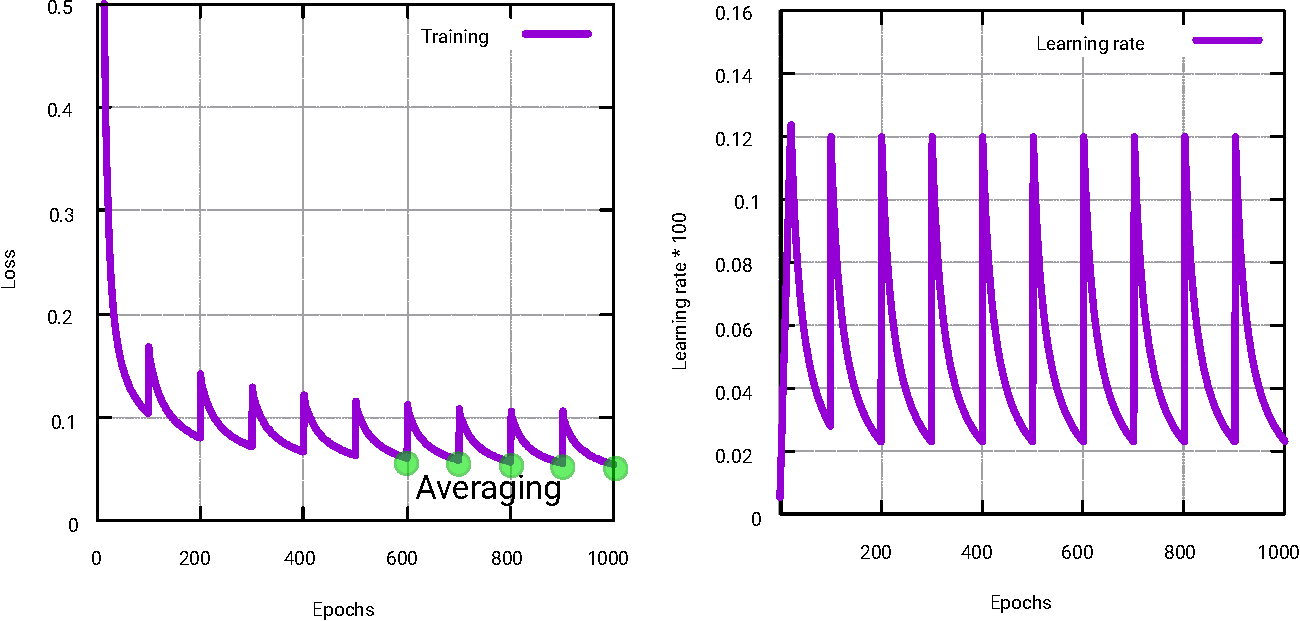
\includegraphics[width = 16.5cm]{images/t3-3.pdf}
  \caption{Learning curves and rate schedule for T3 model. Loss for training on the left, usual learning rate schedule on the right.}
  \label{fig:t11}
\end{figure}

\begin{table}[h!]
\caption{Parameters of T33 run.}
  \centering
  \begin{tabular}{p{8.2cm}p{1.5cm}p{1.5cm}p{1.5cm}p{1.5cm}}
    \toprule
    Parameter & Value & Top-1 & Top-3 & Top-5 \\
    \midrule
    Last training loss & 0.05491 & & & \\
    \midrule
    \multicolumn{5}{l}{\textbf{Averaging 6-7-8-9-10}} \\ \midrule
    Greedy search  & & 40.62 & & \\
    Beam, T = 1.0  & & 42.24 & 63.25 & 69.38  \\
    Beam, T = 1.3 & & 42.96 & \textbf{64.34} & 69.70 \\ 
    \midrule
    \multicolumn{5}{l}{Averaging 7-8-9-10} \\ \midrule
    Greedy search  & & 40.42 & & \\
    Beam, T = 1.0  & & 42.00 & 63.22 & 69.40  \\
    Beam, T = 1.3 & & 42.76 & 64.20 & 69.80 \\ \midrule
    \multicolumn{5}{l}{Averaging 8-9-10} \\ \midrule
    Greedy search  & & 40.38 & & \\
    Beam, T = 1.0  & & 41.84 & 62.96 & 69.08  \\
    Beam, T = 1.3 & & 42.54 & 63.97 & 69.64 \\ \midrule
    \multicolumn{5}{l}{Averaging 9-10} \\ \midrule
    Greedy search  & & 40.20 & & \\
    Beam, T = 1.0  & & 41.86 & 62.56 & 68.30  \\
    Beam, T = 1.3 & & 42.62 & 63.39 & 69.12 \\ 
    \bottomrule
  \end{tabular}
  \label{tbl:t33}
\end{table} 

Model with weights averaging 6-7-8-9-10:

\url{https://github.com/bigchem/retrosynthesis/papers/retrosynthesis/models/t3-3.h5}


\end{document}
